
\documentclass[a4paper,12pt]{article}
\usepackage{enumitem} % -> Alphabetical Lists
\usepackage{amsmath} % -> Matrices
\usepackage{fullpage} % -> A4 Full Page
\usepackage{amssymb} % -> Therefore
\usepackage[utf8]{inputenc}
\usepackage{graphicx}
\usepackage{adjustbox}
\usepackage{listings}
\usepackage{braket}
\usepackage{geometry}
\usepackage{tikz}
\usepackage{gensymb}

\usetikzlibrary{quantikz}

\graphicspath{ {./} }

\geometry{
    a4paper,
    total={170mm,257mm},
    left=20mm,
    top=20mm,
}

\title{Quantum Computing Assignment 7 - Group 18}
\author{
    Rallabhandi, Anand Krishna 
    \and
    Mustafa, Syed Husain
    \and
     , Mohammed Kamran 
}
\date{\today}

\begin{document}

\maketitle

\section*{Exercise 7.1}

 \begin{large}(\textbf{Schmidt Decomposition \& Schr{\"o}dinger Equation})
 \end{large}

\begin{enumerate}[label=(\alph*)]
\item

\underline{Part 1}
\begin{gather*}
     |\psi\rangle = \frac{1}{\sqrt{2}}*(|00\rangle + |11\rangle)\\~\\
     |\psi\rangle = \sum A_{ij}|ij\rangle\\~\\
     A  =  \frac{1}{\sqrt{2}}*  \begin{bmatrix}
1 & 0 \\
0 & 1
\end{bmatrix}\\~\\
svd(A) =\frac{1}{\sqrt{2}}* \begin{bmatrix}
-1 & 0 \\
0 & -1
\end{bmatrix} * \begin{bmatrix}
1 & 0 \\
0 & 1
\end{bmatrix} * \begin{bmatrix}
-1 & 0 \\
0 & -1
\end{bmatrix}
\end{gather*}
Schmidt decomposition is 
\begin{gather*}
    |\psi\rangle = \sum \lambda_\alpha * |\psi_{A,\alpha}\rangle * |\psi_{B,\alpha}\rangle \\~\\
    = \begin{bmatrix}
|\psi_{A,0}\rangle |\psi_{A,1}\rangle \\
\end{bmatrix} * 
\begin{bmatrix}
\lambda_0 & 0 \\
 0 & \lambda_1
\end{bmatrix} *
\begin{bmatrix}
|\psi_{A,0}\rangle |\psi_{A,1}\rangle \\
\end{bmatrix} \\~\\
= \frac{1}{\sqrt{2}}\begin{bmatrix}
-|0\rangle & -|1\rangle \\
\end{bmatrix} * 
\begin{bmatrix}
1 & 0 \\
 0 & 0
\end{bmatrix} *
\begin{bmatrix}
-|0\rangle\\
-|1\rangle \\
\end{bmatrix} \\~\\
\end{gather*}

\underline{Part 2}
\begin{gather*}
    |\psi\rangle = \frac{1}{2}*(|00\rangle + |01\rangle + |10\rangle+ |11\rangle)\\~\\
     A  =  \frac{1}{2}*  \begin{bmatrix}
1 & 1 \\
1 & 1
\end{bmatrix}\\~\\
svd(A) =\frac{1}{\sqrt{2}}* \begin{bmatrix}
1 & 1 \\
1 & -1
\end{bmatrix} * \begin{bmatrix}
1 & 0 \\
0 & 0
\end{bmatrix} * \frac{1}{\sqrt{2}} *  \begin{bmatrix}
1 & 1 \\
1 & -1
\end{bmatrix}
\end{gather*}
Schmidtt decomposition is 
\begin{gather*}
    |\psi\rangle = \sum \lambda_\alpha * |\psi_{A,\alpha}\rangle * |\psi_{B,\alpha}\rangle \\~\\
    = \begin{bmatrix}
|\psi_{A,0}\rangle |\psi_{A,1}\rangle \\
\end{bmatrix} * 
\begin{bmatrix}
\lambda_0 & 0 \\
 0 & \lambda_1
\end{bmatrix} *
\begin{bmatrix}
|\psi_{A,0}\rangle |\psi_{A,1}\rangle \\
\end{bmatrix} \\~\\
\frac{1}{2}\begin{bmatrix}
|0\rangle + |1\rangle & |0\rangle - |1\rangle  \\
\end{bmatrix} * 
\begin{bmatrix}
1 & 0 \\
 0 & 0
\end{bmatrix} *
\begin{bmatrix}
|0\rangle + |1\rangle  \\
|0\rangle - |1\rangle 
\end{bmatrix} \\~\\
\end{gather*}
\item \phantom{-} \\
    Given $U_{t}=e^{-iHt},$ as $ \hbar = 1 $ \& H =$\begin{pmatrix}
        \omega_{1} & 0 \\
        0 & \omega_{2} \\
    \end{pmatrix}$ \\
    Since H is Hermitian, i.e; $H^{2}=I$\\
    We can use Eq. 2.20, i.e; $e^{iAx} = \cos(x)I + i\sin(x)A$ to represent $U_{t}$ as follows: \\
    \[U_{t} = e^{-iHt} \implies U_{t} = \cos(t)\begin{pmatrix}
        1 & 0 \\
        0 & 1 \\
    \end{pmatrix} -i\sin(t)\begin{pmatrix}
        \omega_{1} & 0 \\
        0 & \omega_{2} \\
    \end{pmatrix}\]\[ \implies \begin{pmatrix}
        cos(t) & 0 \\
        0 & cos(t) \\
    \end{pmatrix} -\begin{pmatrix}
        i\sin(t)\omega_{1} & 0 \\
        0 & i\sin(t)\omega_{2} \\
    \end{pmatrix}\]\\ 
    \[\implies U_{t} =\begin{pmatrix}
        \cos(t) - i\sin(t)\omega_{1} & 0 \\
        0 & \cos(t) - i\sin(t)\omega_{2} \\
    \end{pmatrix} \hspace{5mm} \textbf{(A)}\]\\
    Using \textbf{(A)} we can solve for $\ket{\psi(t)}$ given $\ket{\psi(0)}$.\\~\\
    \emph{(i)} $\ket{\psi(0)} = \ket{0}$ \\~\\
    $\implies \ket{\psi(t)} = \begin{pmatrix}
        \cos(t) - i\sin(t)\omega_{1} & 0 \\
        0 & \cos(t) - i\sin(t)\omega_{2} \\
    \end{pmatrix}\begin{pmatrix}
        1 \\
        0 \\
    \end{pmatrix}$\\ $\implies \ket{\psi(t)}  = \Big(\cos(t) - i\sin(t)\omega_{1} \Big)\ket{0}\pagebreak$ \\
    \emph{(ii)} $\ket{\psi(0)} = \frac{1}{\sqrt{2}}\Big(\ket{0}+\ket{1}\Big)$ \\~\\
    $\implies \ket{\psi(t)} = \frac{1}{\sqrt{2}} \begin{pmatrix}
        \cos(t) - i\sin(t)\omega_{1} & 0 \\
        0 & \cos(t) - i\sin(t)\omega_{2} \\
    \end{pmatrix} \begin{pmatrix}
        1 \\
        1 \\ 
    \end{pmatrix}$\\ 
    $\implies \ket{\psi(t)} = \frac{1}{\sqrt{2}}\begin{pmatrix}
        \Big(\cos(t) - i\sin(t)\omega_{1}\Big)\ket{0} +  \Big(\cos(t) - i\sin(t)\omega_{2}\Big)\ket{1}
    \end{pmatrix}$ \\~\\
\item \phantom{-} 
    Given H=$\begin{pmatrix}
        \omega_{1} & 0 \\
        0 & \omega_{2} \\
    \end{pmatrix} + \epsilon\begin{pmatrix}
        0 & 1 \\
        1 & 0 \\
    \end{pmatrix}$ \\~\\
    This can be re-written as: 
    \[H= \bar{w}\begin{pmatrix}
        1 & 0 \\
        0 & 1 \\
    \end{pmatrix} + \vartriangle\omega\begin{pmatrix}
        1 & 0 \\
        0 & -1 \\
    \end{pmatrix} + \epsilon \begin{pmatrix}
        0 & 1 \\
        1 & 0 \\
    \end{pmatrix} \equiv \bar{\omega}I + \sqrt{\vartriangle\omega^{2} + \epsilon^{2}}(\vec{v}.\vec{\sigma})\]
    Where $\bar{\omega}$ is assumed to be $\frac{\omega_{1}+\omega_{2}}{2}$ \& $\vartriangle\omega = \frac{\omega_{1} - \omega_{2}}{2}$\\~\\
    $\implies Ht = \bar{w}tI + \vartriangle\omega tZ  + \epsilon tX \implies e^{-iHt} = e^{-i\bar{\omega}tI -i\vartriangle \omega tZ  -i\epsilon t X} \approx \underbrace{e^{-i(\bar{w}t)I}}_{\textbf{(A)}}.\underbrace{e^{-i(\vartriangle \omega t) Z}}_{\textbf{(B)}}.\underbrace{e^{-i(\epsilon t)X}}_{\textbf{(C)}}$\\~\\ \phantom{-} \\
    Using Eq. 2.20 in \textbf{(A)} $:\begin{pmatrix}
        \cos(\bar{w}t) & 0 \\
        0 & \cos(\bar{w}t) \\
    \end{pmatrix} - \begin{pmatrix}
        i\sin(\bar{w}t) & 0 \\
        0 & i\sin(\bar{w}t) \\
    \end{pmatrix} = \begin{pmatrix}
        e^{-i(\bar{w}t)} & 0 \\
        0 & e^{-i(\bar{w}t)} \\
    \end{pmatrix}$ \\~\\
    Using Eq. 2.20 in \textbf{(B)} $:\begin{pmatrix}
        \cos(\vartriangle \omega t) - i\sin(\vartriangle \omega t) & 0 \\
        0 & \cos(\vartriangle \omega t) +i\sin(\vartriangle \omega t)  \\
    \end{pmatrix} = \begin{pmatrix}
        e^{-i(\vartriangle\omega t)} & 0 \\
        0 & e^{i(\vartriangle\omega t)} \\
    \end{pmatrix}$ \\~\\
    Using Eq. 2.20 in \textbf{(C)}: $\begin{pmatrix}
        \cos(\epsilon t) & -i\sin(\epsilon t) \\
        -i\sin(\epsilon t) & \cos(\epsilon t) \\
    \end{pmatrix}$ \\~\\
    $\implies U_{t} = e^{-iHt} \approx \textbf{(A)(B)(C)}$ \\~\\ 
    $\textbf{(A)(B)} : \begin{pmatrix}
        e^{-i(\bar{w}t)} & 0 \\
        0 & e^{-i(\bar{w}t)} \\
    \end{pmatrix}\times \begin{pmatrix}
        e^{-i(\vartriangle\omega t)} & 0 \\
        0 & e^{i(\vartriangle\omega t)} \\
    \end{pmatrix}  = \begin{pmatrix}
        e^{-i(\bar{\omega} +\vartriangle \omega)t} & 0 \\
        0 & e^{i(\vartriangle \omega -\bar{\omega})t}
    \end{pmatrix} = \begin{pmatrix}
        e^{-i(\omega_{1})t} & 0 \\
        0 & e^{-i(\omega_{2})t} \\
    \end{pmatrix}$ \\~\\ \phantom{-} \\
    $U_{t} =  \begin{pmatrix}
        e^{-i(\omega_{1})t} & 0 \\
        0 & e^{-i(\omega_{2})t} \\ 
    \end{pmatrix} \times \begin{pmatrix}
        \cos(\epsilon t) & -i\sin(\epsilon t) \\
        -i\sin(\epsilon t) & \cos(\epsilon t) \\
    \end{pmatrix} = \begin{pmatrix}
        e^{-i(\omega_{1})t}\cos(\epsilon t) & -ie^{-i(\omega_{1})t}\sin(\epsilon t) \\
        -ie^{-i(\omega_{2})t}\sin(\epsilon t) & e^{-i(\omega_{2})t}\cos(\epsilon t) \\ 
    \end{pmatrix} $ \\~\\
    $\ket{\psi(t)} = U_{t}\ket{0} \implies \ket{\psi(t)} = \begin{pmatrix}
        e^{-i(\omega_{1})t}\cos(\epsilon t) \\
        -ie^{-i(\omega_{2})t}\sin(\epsilon t) \\
    \end{pmatrix}$ \\~\\
    \begin{center}
        $\therefore \braket{1|\psi(t)} = \begin{pmatrix}
            0 & 1 \\
        \end{pmatrix} \begin{pmatrix}
            e^{-i(\omega_{1})t}\cos(\epsilon t) \\
            -ie^{-i(\omega_{2})t}\sin(\epsilon t) \\
        \end{pmatrix} = -ie^{-i(\omega_{2})t}\sin(\epsilon t)$
    \end{center}
    

  

\item
\begin{gather*}
    |\psi(t)\rangle = U_t|\psi(0)\rangle\\~\\
    \rho = \sum_j p_j |\psi_j(t)\rangle \langle\psi_j(t)| = \sum_j p_j  U_t|\psi(0)\rangle \langle\psi(0)| U_t^{\dagger} = U_t A U_t^{\dagger}\\~\\
    U_t= e^{\frac{-iHt}{h}}\\~\\
    \frac{d U_t}{dt} = \frac{-iH}{h}U_t \\~\\
     \frac{d \rho}{d_t} = (\frac{-iHU_t}{h}) *A U_t^{\dagger} +   U_t^{\dagger} A (\frac{i H U_t^{\dagger}}{h})\\~\\
     = \frac{-i}{h}[H \rho - \rho H]\\~\\
     ih \frac{d \rho(t)}{d_t} = [H \rho - \rho H] = [H, \rho(t)]
\end{gather*}
\begin{center}
    Thus the derivation of Von Neumann equation is proved.\\~\\ \pagebreak
\end{center}

\end{enumerate}
\begin{large}(\textbf{Python/Numpy implementation of the partial trace})
\end{large}\\~\\

\begin{enumerate}[label=(\alph*)]
\item \phantom{-} \\~\\  
\graphicspath{./images/}
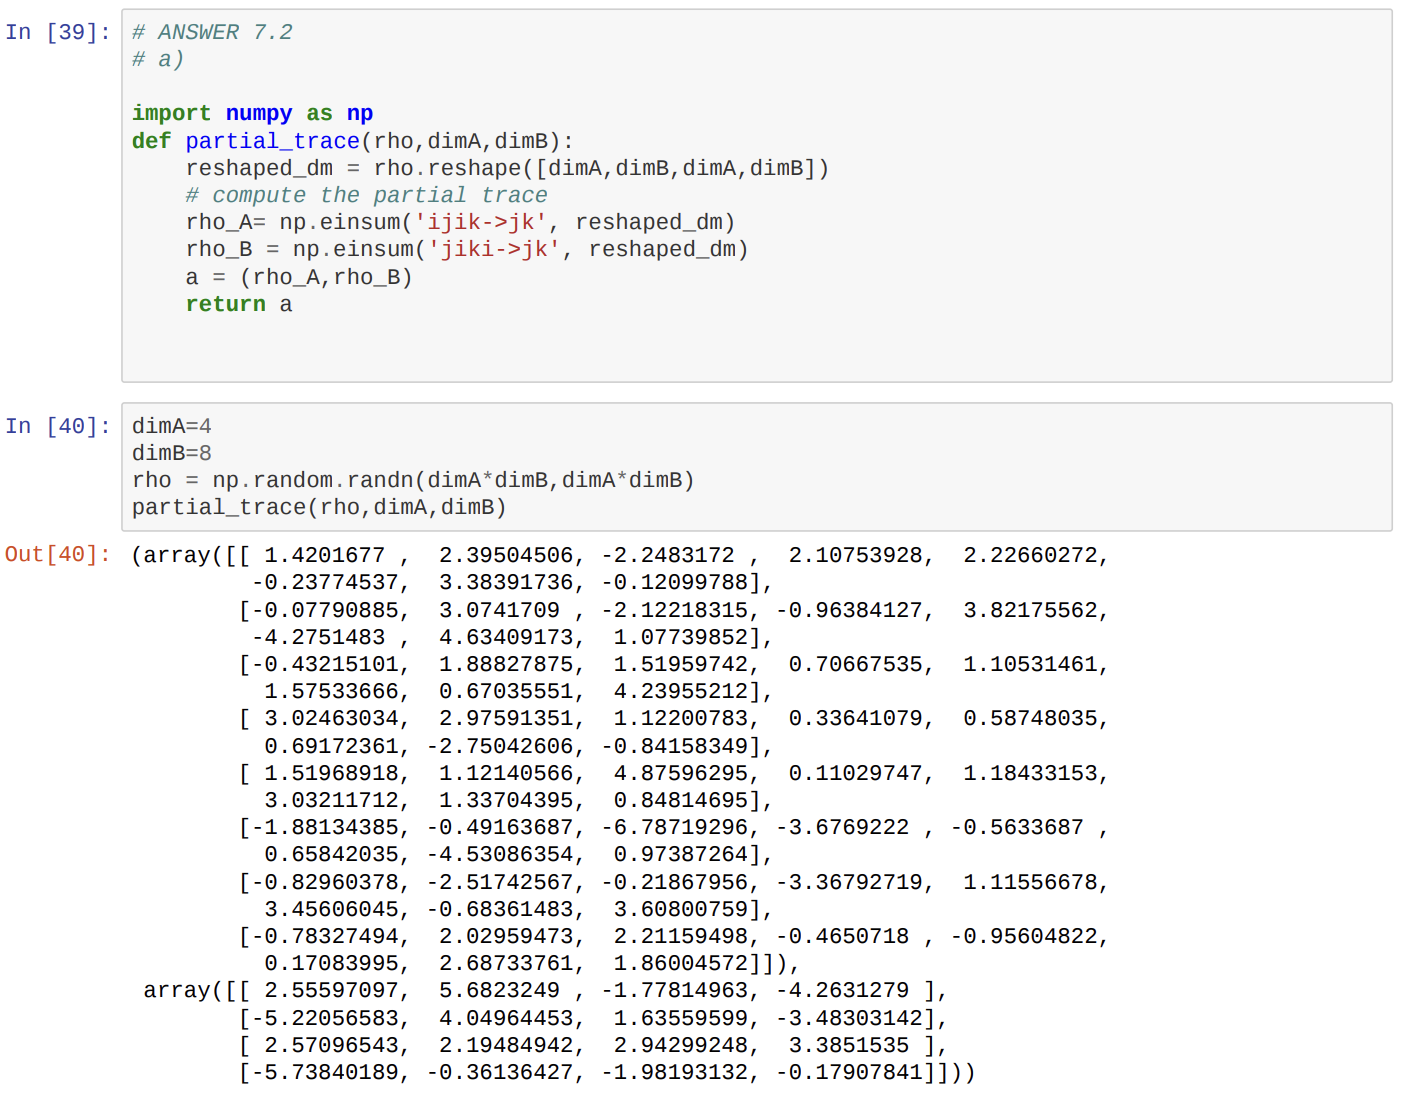
\includegraphics[scale=0.60]{images/1.png}\\~\\
\item \phantom{-} \\~\\
 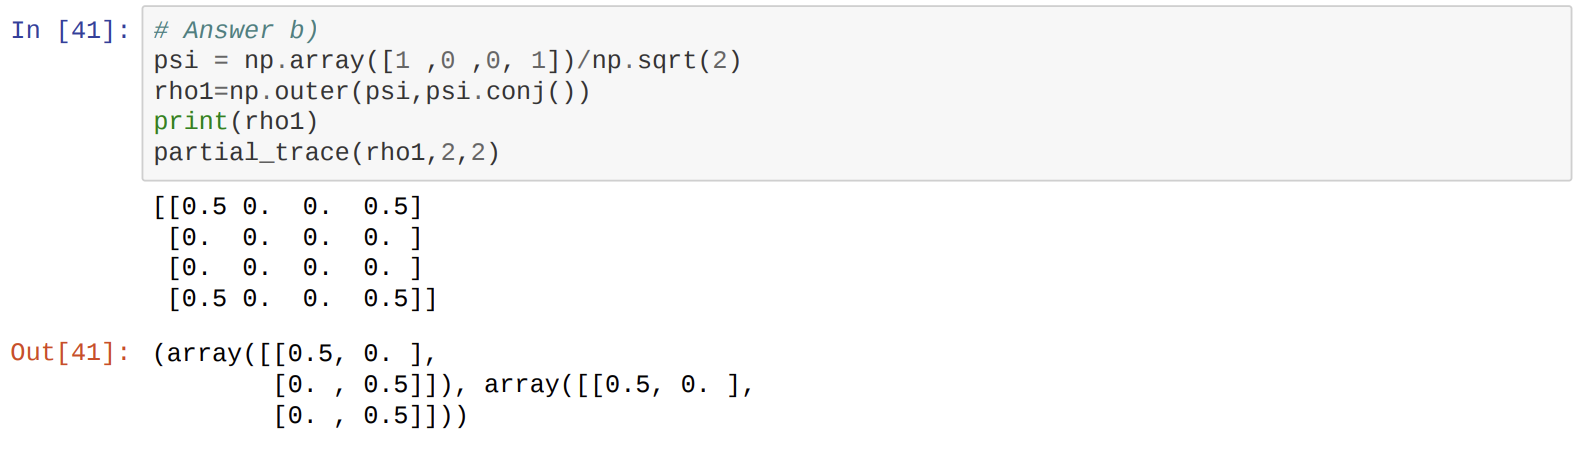
\includegraphics[scale=0.6]{images/2.png}\\~\\
 \pagebreak
\item \phantom{-}\\
 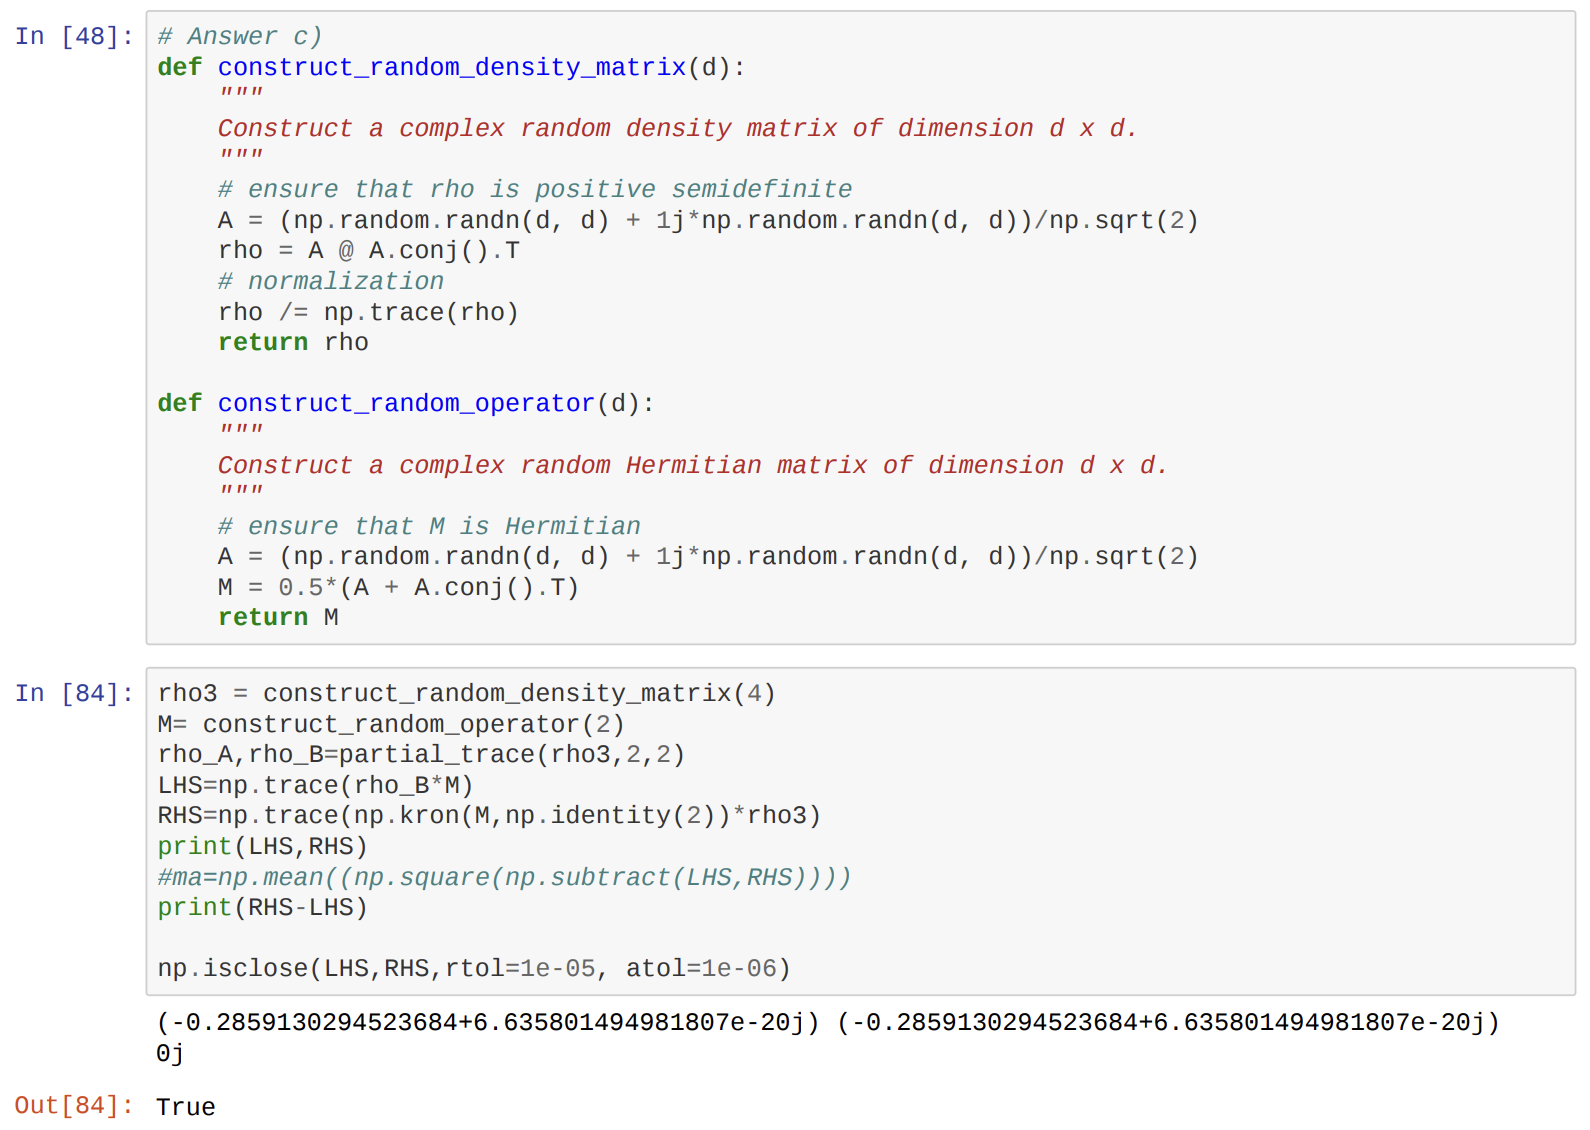
\includegraphics[scale=0.6]{images/3.png}\\
\end{enumerate}
\end{document}
